\section{函数图像}
在初中我们学过一次函数、反比例函数以及二次函数,它们的图像就不再介绍了。如记性不好的去请教初中数学老师。

顺带提一句:下文讲述的函数的绘制方法只能画出近似的、粗略的函数图像,这种精度在绝大多数情况下是没有问题的\footnote{例外情况指方程的解的个数问题,前文已经提过。},您也应该在绝大多数情况下绘制这种图像。

对于三角函数,会在后面的“三角函数”章节提到。这里仅仅画出它们的图像而不研究其性质。

\subsection{耐克函数}
首先介绍的是耐克函数(或称对勾函数),它的解析式形如:\[y=ax+\frac{b}{x}\]

通过描点法,不难画出它的图像(如图\ref{fig:figure-of-tick-functions})。

\begin{figure}[htb]
	\centering
	\begin{subfigure}[b]{0.24\textwidth}
		\centering
		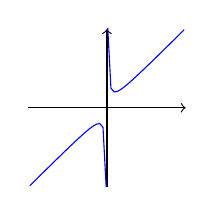
\begin{tikzpicture}[scale=0.1]
			\draw[->] (-10, 0) -- (10, 0);
			\draw[->] (0, -10) -- (0, 10);
			\draw[color=blue, domain=0.1:9.8] plot(\x, \x + 1 / \x);
			\draw[color=blue, domain=-9.8:-0.1] plot(\x, \x + 1 / \x);
		\end{tikzpicture}
		\caption{$y=1+\frac{1}{x}$}
		\label{fig:figure-of-tick-functions-a}
	\end{subfigure}
	\begin{subfigure}[b]{0.24\textwidth}
		\centering
		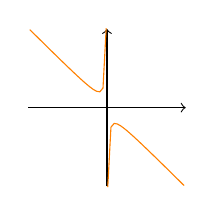
\begin{tikzpicture}[scale=0.1]
			\draw[->] (-10, 0) -- (10, 0);
			\draw[->] (0, -10) -- (0, 10);
			\draw[color=orange, domain=0.1:9.8] plot(\x, -\x - 1 / \x);
			\draw[color=orange, domain=-9.8:-0.1] plot(\x, -\x - 1 / \x);
		\end{tikzpicture}
		\caption{$y=-1-\frac{1}{x}$}
		\label{fig:figure-of-tick-functions-b}
	\end{subfigure}
	\begin{subfigure}[b]{0.24\textwidth}
		\centering
		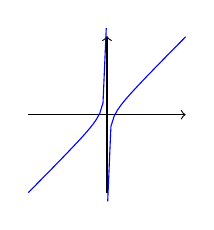
\begin{tikzpicture}[scale=0.1]
			\draw[->] (-10, 0) -- (10, 0);
			\draw[->] (0, -10) -- (0, 10);
			\draw[color=blue, domain=0.09:10] plot(\x, \x - 1 / \x);
			\draw[color=blue, domain=-10:-0.09] plot(\x, \x - 1 / \x);
		\end{tikzpicture}
		\caption{$y=1-\frac{1}{x}$}
		\label{fig:figure-of-tick-functions-c}
	\end{subfigure}
	\begin{subfigure}[b]{0.24\textwidth}
		\centering
		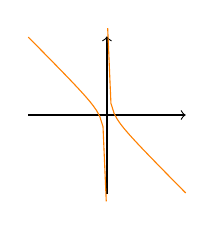
\begin{tikzpicture}[scale=0.1]
			\draw[->] (-10, 0) -- (10, 0);
			\draw[->] (0, -10) -- (0, 10);
			\draw[color=orange, domain=0.09:10] plot(\x, -\x + 1 / \x);
			\draw[color=orange, domain=-10:-0.09] plot(\x, -\x + 1 / \x);
		\end{tikzpicture}
		\caption{$y=-1+\frac{1}{x}$}
		\label{fig:figure-of-tick-functions-d}
	\end{subfigure}
	\caption{参量取不同值时耐克函数的图像}
	\label{fig:figure-of-tick-functions}
\end{figure}

然后我们可以得出耐克函数图像的性质:

\begin{itemlist}
	\item $a^+,b^+$是一、三象限的耐克函数(如图\ref{fig:figure-of-tick-functions-a})
	\item $a^-,b^-$是二、四象限的耐克函数(如图\ref{fig:figure-of-tick-functions-b})
	\item $a^+,b^-$是双增函数(如图\ref{fig:figure-of-tick-functions-c})
	\item $a^-,b^+$是双减函数(如图\ref{fig:figure-of-tick-functions-d})
\end{itemlist}

再看一眼函数图像,$a$、$b$同号时在各个象限内有极值点,接下来将推导出这个点的坐标:

\begin{proof}
	根据基本不等式得:\[ax+\frac{b}{x}\geq2\sqrt{ab}\]

	此时不等号右边即极值点的纵坐标,代入原式解方程:
	\[\begin{split}
		&ax+\frac{b}{x}=2\sqrt{ab} \\
		&ax^2-2x\sqrt{ab}+b=0 \\
		&x=\sqrt{\frac{b}{a}}
	\end{split}\]

	可以得到耐克函数在第一象限内的顶点坐标为$(\sqrt{\frac{b}{a}},2\sqrt{ab})$,其它象限只需在对应的地方添负号即可。
\end{proof}

\subsection{幂函数}
在初中我们学过了反比例函数、二次函数,它们都是幂函数的一种。其解析式为:\[y=x^a(a=\frac{p}{q}\quad p,q\in\mathbb{Z})\]

要绘制幂函数的图像,应把第一象限的图像和其余部分的图像分别绘制。

第一象限的图像如图\ref{fig:figure-of-power-function}所示。

\begin{figure}[htb]
	\centering
	\begin{subfigure}[b]{0.3\textwidth}
		\centering
		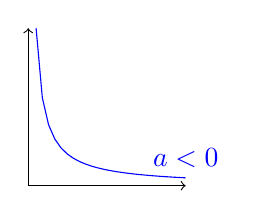
\begin{tikzpicture}[scale=0.2]
			\draw[->] (0, 0) -- (10, 0);
			\draw[->] (0, 0) -- (0, 10);
			\draw[color=blue, domain=0.5:10] plot(\x, 5 / \x) node[above] {$a<0$};
		\end{tikzpicture}
		\caption{减}
	\end{subfigure}
	\begin{subfigure}[b]{0.3\textwidth}
		\centering
		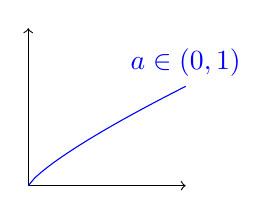
\begin{tikzpicture}[scale=0.2]
			\draw[->] (0, 0) -- (10, 0);
			\draw[->] (0, 0) -- (0, 10);
			\draw[color=blue, domain=0:10] plot(\x, \x ^ 0.8) node[above] {$a\in(0,1)$};
		\end{tikzpicture}
		\caption{缓慢增}
	\end{subfigure}
	\begin{subfigure}[b]{0.3\textwidth}
		\centering
		\begin{tikzpicture}[scale=0.2]
			\draw[->] (0, 0) -- (10, 0);
			\draw[->] (0, 0) -- (0, 10);
			\draw[color=blue, domain=0:6.81] plot(\x, \x ^ 1.2) node[right] {$a>1$};
		\end{tikzpicture}
		\caption{快速增}
	\end{subfigure}
	\caption{幂函数第一象限内的图像}
	\label{fig:figure-of-power-function}
\end{figure}

其它象限的图像可按照下面的流程绘出:
\[\begin{cases}
	\text{$q$为偶数} & \text{只有第一象限图像} \\
	\text{$q$为奇数} & \text{判断$p$}
	\begin{cases}
		\text{$p$为奇数} & \text{函数为奇函数} \\
		\text{$p$为偶数} & \text{函数为偶函数}
	\end{cases}
\end{cases}\]
